% Chapter Template

\chapter{Literature Review} % Main chapter title

\label{LiteratureReview} % Change X to a consecutive number; for referencing this chapter elsewhere, use \ref{ChapterX}

%----------------------------------------------------------------------------------------
%	Image Classification
%----------------------------------------------------------------------------------------
\section{Image Classification}

Image classification is the precursor problem to action recognition. Without the ability to classify individual images, the ability to classify videos, which functionally are a list of individual images, would never have been researched as nearly every technique for action recognition can be tracked from some form of image classification task.

An example of this task is the CIFAR dataset \cite{cifar}, where the goal is to simply classify relatively low resolution images into either 10 or 100 classes, depending on the version of the dataset. This dataset is very well explored, and results have high 90\% accuracy values through very complex models and modern techniques. However, some simple models such as EfficientNet \cite{efficientnet} are able to achieve this above 90\% metric while providing a model that is efficient and able to train and evaluate images quickly. The popularization of image classification led to the popularization of CNN's which are also actively used in action recognition, and particularly popular in intermediate representation models that will be discussed in section \ref{sec:intermediate}.

%----------------------------------------------------------------------------------------
%	Optical Flow
%----------------------------------------------------------------------------------------
\section{Optical Flow}

Optical Flow, not dissimilar to pose estimation described in section \ref{sec:pose-detection}, is something that is often taken for granted in models that utilize it, however it can be computed in several different ways. An example of an optical flow technique is the method utilized by the I3D model \cite{i3d} which will be discussed later in this chapter. This technique is known as TV-L optical flow \cite{TV-L}, and utilizes a formula based on the total variation (TV) regularization and the robust $L^1$ norm in the data fidelity term. While the methods described in this paper and many others are rather complex, the idea that provides performance improvements is that optical flow represents the movement of a person from one frame to another and eliminating background information which does not move, this is further demonstrated in figure \ref{fig:opticalflow}.

\begin{figure}[ht]
	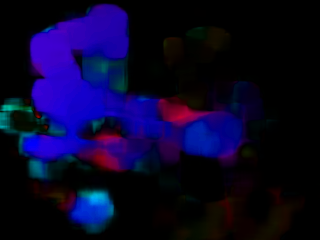
\includegraphics[width=10cm]{opticalflow}
	\centering
	\caption{An example of the optical flow field \textbf{(c)}, resultant from the first and second frames \textbf{(a)} \textbf{(b)}. The goal being that the background is not in the optical flow field, only the movement of subjects in the frames are considered. This particular example is utilizing the TV-L optical flow \cite{TV-L}.}
	\label{fig:opticalflow}
\end{figure}

%----------------------------------------------------------------------------------------
%	Convolutional Neural Networks
%----------------------------------------------------------------------------------------

\section{Convolutional Neural Networks}

Convolutional Neural Networks are a key part of both this thesis and the larger domain of computer vision. Using these models, computer vision took a large step forward in the domain of image processing, and is still being developed by modern models in order to extract further performance \cite{deeplearning}.

\subsection{Structure}

The classic structure of a convolutional neural network can be studied through one of the first recognizable architectures LeNet-5 \cite{lenet5}, as shown in figure \ref{fig:lenet5}. This architecture is broken into a few key layers that are common in CNN's used even today:

\begin{itemize}
	\item Convolutions
	\item Subsampling
	\item Flatten
	\item Fully Connected
\end{itemize}

\begin{figure}[ht]
	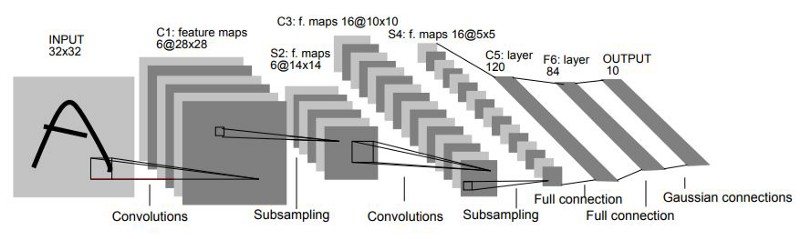
\includegraphics[width=1\textwidth]{LeNet5}
	\centering
	\caption{Classical LeNet-5 architecture \cite{lenet5} containing convolutional, subsampling, and fully connected layers.}
	\label{fig:lenet5}
\end{figure}

The \textbf{convolutions} are the key part of how convolutional neural networks function, and they function using a \textbf{kernel}. This kernel is built as an $NxN$ matrix of randomly initialized values, this matrix is then 'slid' across the entire image, and the values that the kernel 'sits on top' of are multiplied by the kernel values and then summed to produce an output cell in the output image. An example of a $4x4$ greyscale image and $2x2$ kernel is shown in figure \ref{fig:kernel-example}. In addition to this process, sometimes the edges of images are 'padded' with zeroes in order to avoid the reduction in image size when a kernel reaches the edge of an image. This kernel can also be expanded to 3 dimensions in order to be utilized on video data rather than image data. This functionally works the same as 2-dimensional convolutions, sliding in three directions instead of two, however it results in much larger kernels that take up significantly larger portions of memory. This is because the back-propogation data must be then stored for 27 kernel data points rather than 9 (in the case of a $3x3$ convolution).

\begin{figure}[ht]
	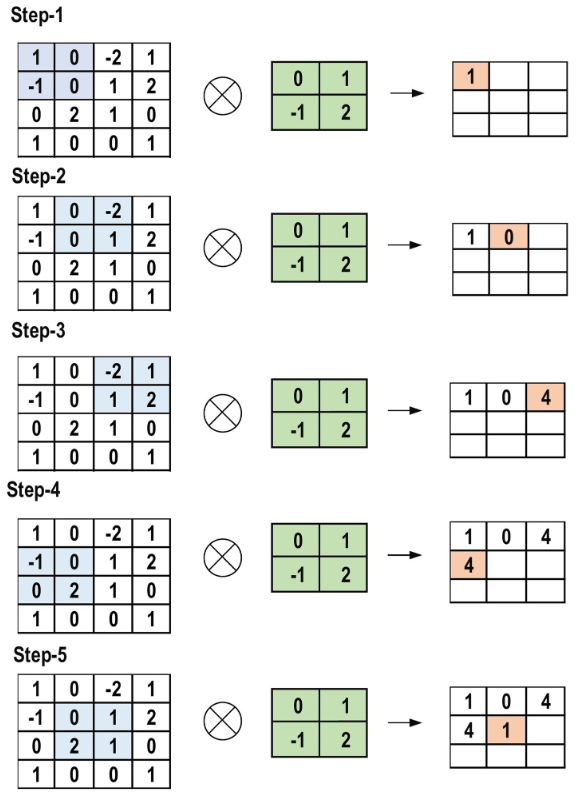
\includegraphics[width=0.7\textwidth]{KernelExample}
	\centering
	\caption{Example of kernel function as shown in Review of Deep Learning: Concepts, CNN architectures, challenges, applications, future directions \cite{2021cnnreview}.}
	\label{fig:kernel-example}
\end{figure}

\subsection{Classic Architectures}
\label{sec:classic-cnn}

\textbf{AlexNet} \cite{alexnet} is another common CNN architecture not dissimilar to the LeNet architecture \cite{lenet5} shown previously in this chapter. AlexNet provided two main contributions over the LeNet architecture. First, it provides a new method of training models on GPU, which involves splitting the parts of the model to be trained separately on different GPU's which can then be combined at the end (as shown in figure \ref{fig:alexnet}), which allowed more GPU memory to be utilized when training the model. Second, it provides a much deeper CNN architecture, where the LeNet architecture contains 2 convolutional layers, the AlexNet architecture contains 5 total convolutional layers, three of which are stacked one after another after the second max pool layer. At the time of writing, AlexNet was the state-of-the-art CNN for image classification and opened new doors with efficient multi-gpu trained models.

\begin{figure}[ht]
	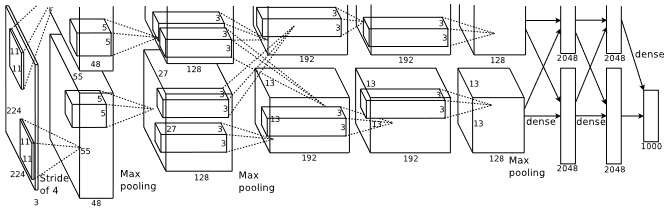
\includegraphics[width=0.7\textwidth]{AlexNet}
	\centering
	\caption{AlexNet \cite{alexnet} CNN architecture as it appears in the original paper \cite{alexnet}. The model is split into two separate top \& bottom parts which are fed through individual GPU's and combined at the end.}
	\label{fig:alexnet}
\end{figure}

\textbf{VGG-16} \cite{vgg16} is another deep convolutional neural network model, again similar to those described previously in this section, however as AlexNet \cite{alexnet} built complexity on top of LeNet \cite{lenet5}, VGG-16 seeks to do the same over AlexNet. The '16' part of VGG-16 refers to the number of convolutional layers, which is much more than the 5 present in AlexNet. While this added complexity is important, VGG-16 also focuses on keeping the individual parts simple, for each of their convolutional layers, the kernel is 3x3 with stride 1, and for each of the pooling layers, they utilize a 2x2 filter with stride 2. These convolutions are split into five different 'blocks' shown in figure \ref{fig:vgg16}, which are separated by these pooling layers, ending with the same dense layers present in AlexNet.

\begin{figure}[ht]
	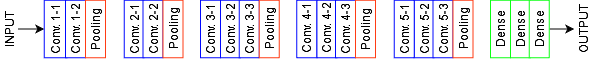
\includegraphics[width=0.9\textwidth]{vgg16}
	\centering
	\caption{VGG-16 \cite{vgg16} architecture, with 16 convolutional layers, each block being separated by pooling layers, ending with three dense layers which provide output.}
	\label{fig:vgg16}
\end{figure}

\subsection{Modern Architectures}

\textbf{ResNet}

\textbf{Residual Attention Network}

%----------------------------------------------------------------------------------------
%	CNN Models
%----------------------------------------------------------------------------------------
\section{CNN Based Models}

Naturally, the first approach to feeding video data into models is to process the raw RGB frames. This technique is derived from image classification tasks, where lightweight and relatively simple CNN's have been shown to have good performance when classifying single images. The logic would then follow that these types of models may be able to classify videos, however they must be modified a few different ways, which will be described further in this chapter.

%----------------------------------------------------------------------------------------
%	CNN + LSTM
%----------------------------------------------------------------------------------------
\subsection{CNN + LSTM Models}

In very classic models, utilizing existing CNN architectures is a very simple process. The individual frames are passed through the CNN model, producing a feature map for each frame. These feature maps are then pooled and passed into dense layers which produces an output. While very simple and fast, this model completely ignores any temporal activity, meaning that the model cannot determine how a person moves throughout a video from one frame to another. This would make differentiating some reversible actions such as running forwards vs running backwards very difficult.

Figure \ref{fig:cnn-lstm} shows the typical modern structure for this solution. After the features are extracted from each of the 2 dimensional CNN, they are passed through a LSTM. The goal of this LSTM module is to carry features from one frame to another and add some temporal element.

\begin{figure}[ht]
	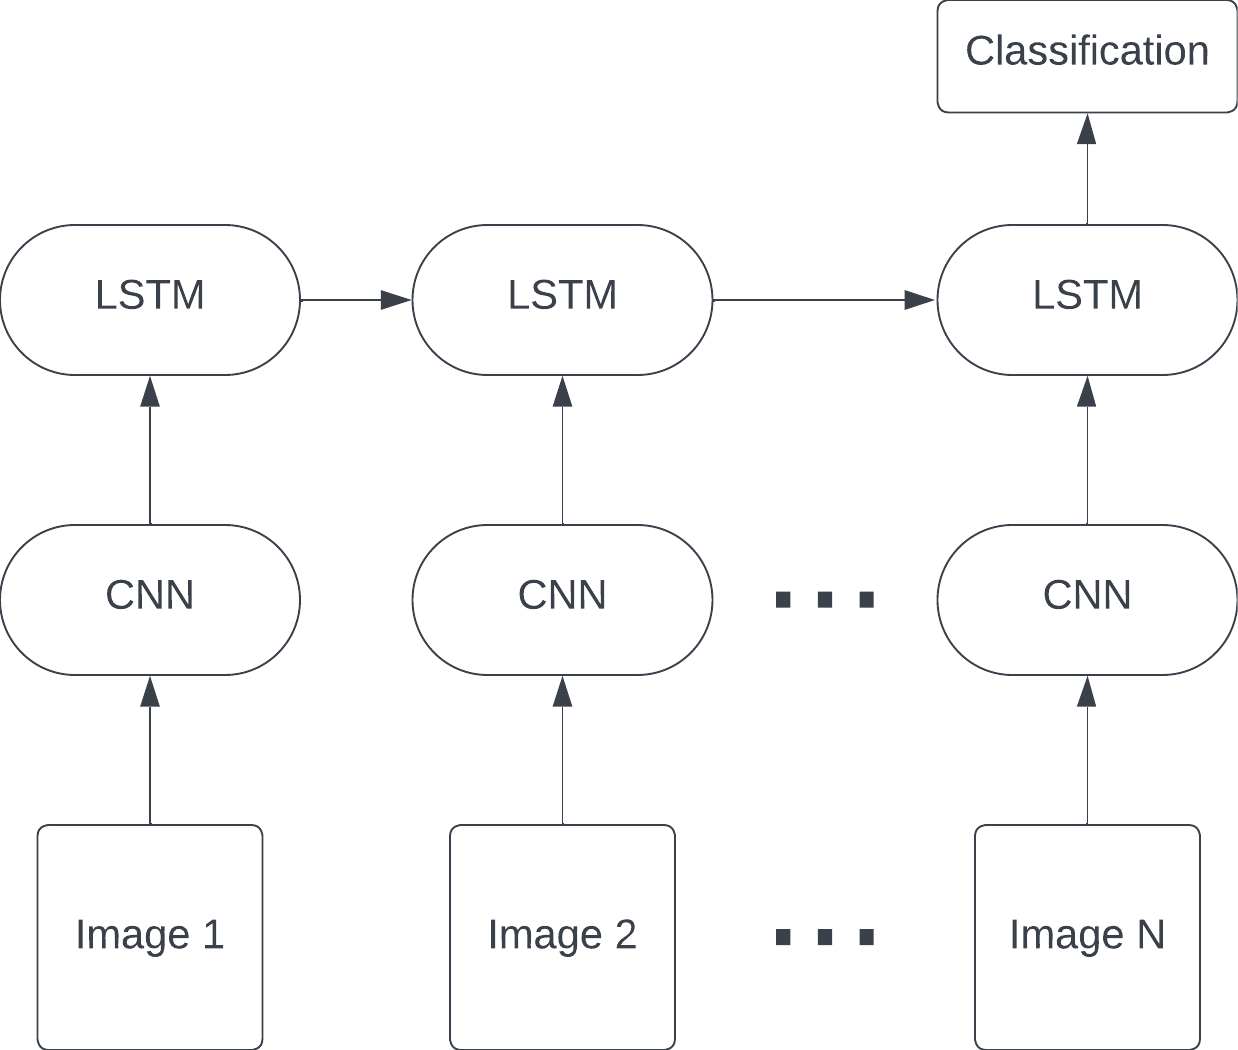
\includegraphics[width=8cm]{CNN-LSTM.png}
	\centering
	\caption{An example structure of a simple CNN-LSTM based model, each individual frame being individually fed into the CNN, and then passed to a LSTM.}
	\label{fig:cnn-lstm}
\end{figure}

The advantages of this model are that is is very lightweight and all of the individual parts are already well studied and efficient. This also means that the models are very lightweight, and relatively simple in comparison to more complex techniques.

The disadvantages of the model are also rooted in it's simplicity. The result of processing each image independently means that the interactions between frames is not very well represented. While the model is able to represent individual frame features very well, due to the fact that the feature maps are passed through the LSTM, classes that require specific movement from one frame to another are difficult to represent using this structure. Constructing these individual feature maps can also fall victim to background interference, meaning that a movement in the camera, or change in background could impact in a way that detracts from the main subject of the action more with this model than the other approaches discussed later in this chapter.

\begin{figure}[ht]
	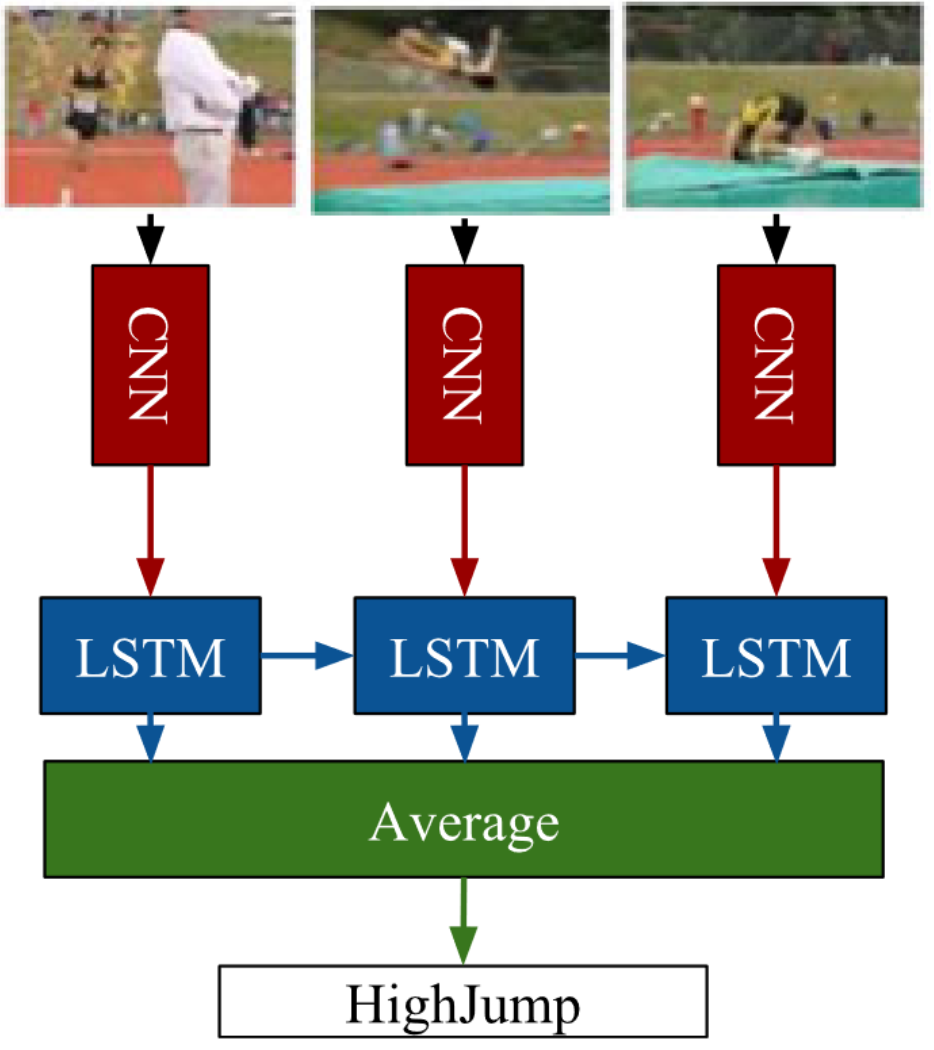
\includegraphics[width=8cm]{LRCN-AR.png}
	\centering
	\caption{Action recognition structure for the LRCN model. \cite{LRCNS}}
	\label{fig:lrcn-ar}
\end{figure}

\textbf{Long-term Recurrent Convolutional Networks} \cite{LRCNS}, is a model constructed using this methodology. In the paper, they use the notation that each frame, $x_{i}$, is fed into the CNN in order to construct a fixed-length feature representation, $\phi_{v}(x_{i})$. This is then passed into the recurrent sequence learning model. This is where the model differs from the previous example provided. In the LRCN model, the LSTM outputs at each frame are averaged to get the output class, rather than taking the last output. This removes any bias the model may have towards the later frames in long videos. In addition to RGB frames, this model additonally uses the optical flow feature, which easily adapts to this structure, replacing the RGB frames in figure \ref{fig:lrcn-ar}. The LSTM structure is taken from \cite{LSTM-2015}, which is a structure devised from the original LSTM model, as we discussed in section \ref{sec:LSTM}. The CNN's, represented in the paper as $\phi$, is described as a hybrid of the CaffeNet \cite{caffenet} (a variant of the AlexNet \cite{alexnet} model discussed in section \ref{sec:classic-cnn}) and the Zeiler and Fergus \cite{zeilerfergus} models, which has been pre-trained on a large dataset.

\begin{figure}[ht]
	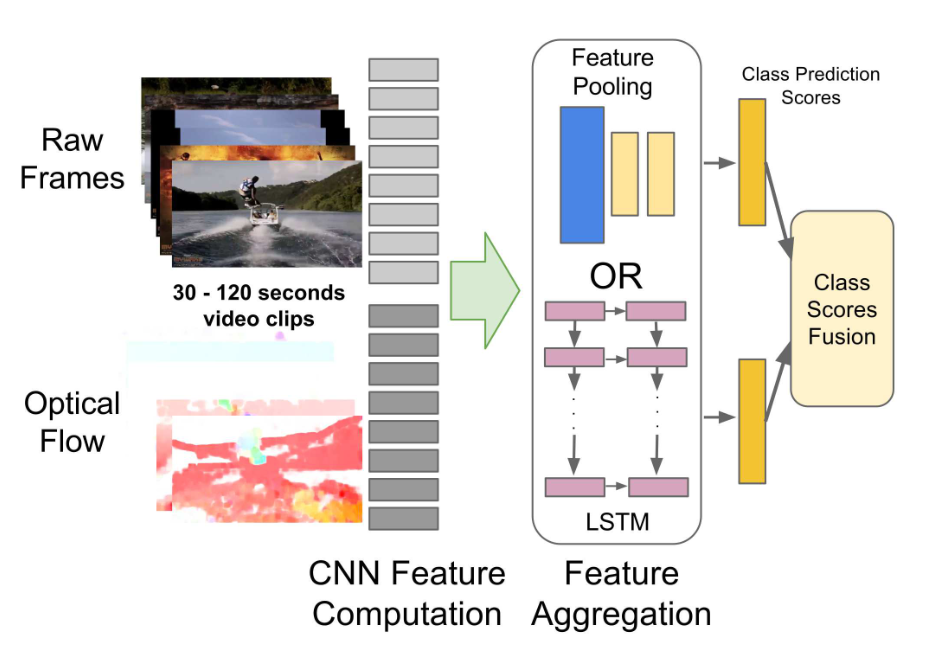
\includegraphics[width=10cm]{BeyondOverview.png}
	\centering
	\caption{Overview of the Beyond Short Snippets: Deep Networks for Video Classification model \cite{beyondshortsnippets}}
	\label{fig:beyondoverview}
\end{figure}

\textbf{Beyond Short Snippets: Deep Networks for Video Classification} \cite{beyondshortsnippets}, is another approach to this structure, which explores a more complex deep-LSTM based module, as well as more classical feature pooling. Similarly to the previously discussed model, Long-term Recurrent Convolutional Networks \cite{LRCNS}, the model utilizes a combination of two popular CNN models, AlexNet \cite{alexnet} and GoogLeNet \cite{googlenet}. The paper did explore many more classical feature pooling architectures, and were proven to have good results, however these techniques were outperformed by the LSTM model. The paper utilized a deep LSTM architecture for the feature aggregation step, shown in figure \ref{fig:deeplstm}, which further adds to it's complexity, moving it above the CNN-LSTM architectures described previously. In this deep-LSTM module, the outputs of each frame are passed into a LSTM module as in the previous model, but the ouputs are then passed up through 4 more stacked layers of LSTM's, after reaching softmax layers which are averaged to get an output. These 4 additional layers of LSTM's mean it is more able to infer data moving from one frame to another. This model additionally explored the uses of optical flow and found that it adds a great deal to the accuracy of the model.

\begin{figure}[ht]
	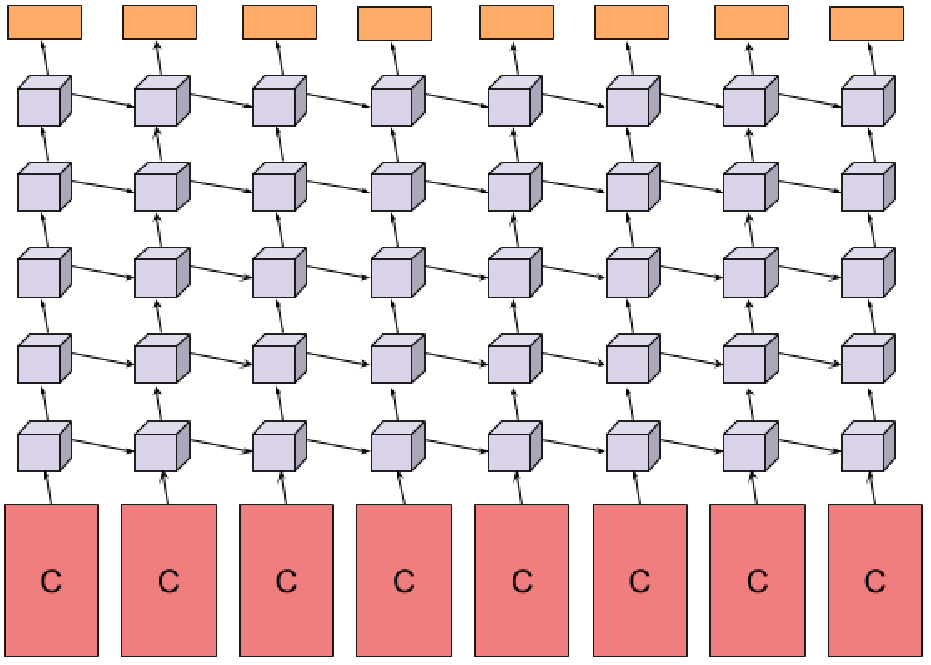
\includegraphics[width=8cm]{deepLSTM.png}
	\centering
	\caption{Deep LSTM architecture utilized by \cite{beyondshortsnippets} in the feature aggregation step as shown in figure \ref{fig:beyondoverview}.}
	\label{fig:deeplstm}
\end{figure}

%----------------------------------------------------------------------------------------
%	3D CNN
%----------------------------------------------------------------------------------------
\subsection{3D CNN Models}
\label{sec:3dCNNModels}

When considering how to handle videos without the LSTM component, the one of the first approaches that was developed is to utilize 3 dimensional CNN kernels, the specifics of which were described in section \ref{3dkernels}. The function of these kernels when it relates to action recognition is that they allow for the model to easily encode local temporal data using the third kernel dimension. The primary issue with these models is that they contain many more parameters over the 2D CNN models, meaning that they take longer to train and require more computing power as compared to the lightweight counterparts.

\textbf{3D Convolutional Neural Networks for Human Action Recognition} \cite{3DCNN-ActionRecognition} was one of the original papers that proposed this model for the purposes of action recognition, and the greater topic of 3 dimensional convolutions as described in section \ref{3dkernels}. The general architecture of the model is shown in figure \ref{fig:original3dcnn}, and is extremely similar to that of 2 dimensional CNNs, with convolutional layers which are followed by subsampling layers.

\begin{figure}[ht]
	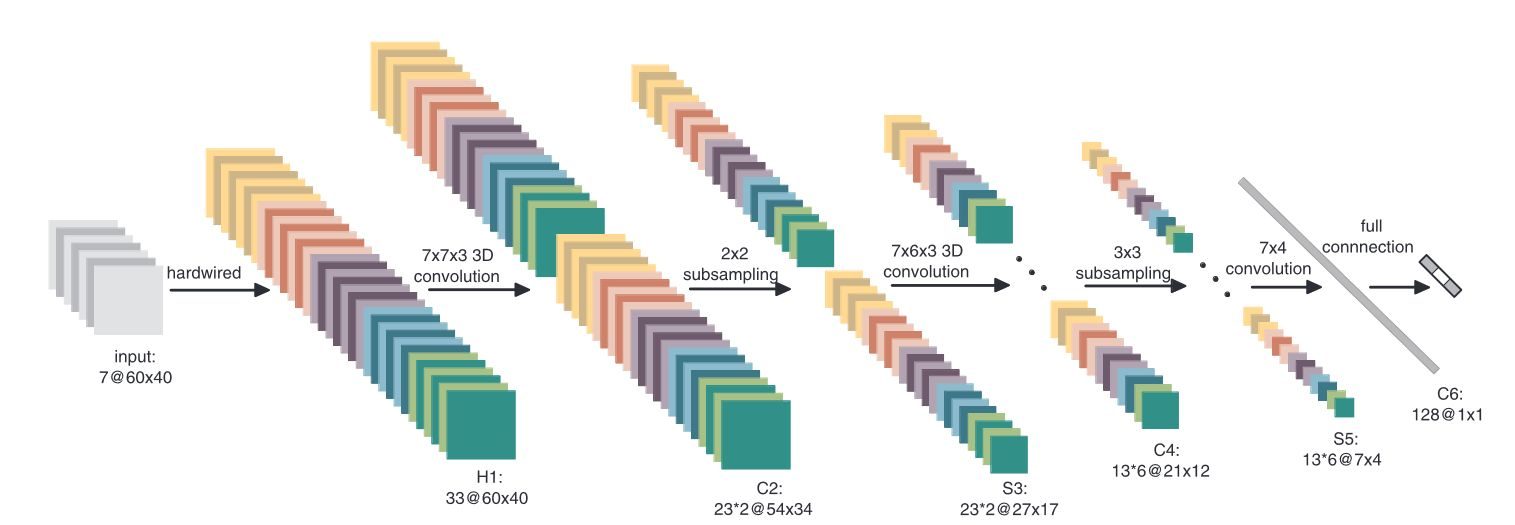
\includegraphics[width=10cm]{og3dCNN}
	\centering
	\caption{The original 3D-CNN action recognition model architecture proposed by \cite{3DCNN-ActionRecognition}, containing 3 convolutional layers, two subsampling layers, and one fully connected layer}
	\label{fig:original3dcnn}
\end{figure}

The primary difference with this original architecture compared to 2D CNN's as we know them today is that it used rather large $7x7x3$ convolutions, as compared to the typical $3x3$ convolutions used in classical 2D CNN's. \textbf{Learning Spatiotemporal Features with 3D Convolutional Networks} \cite{3x33dcnn} is a slightly more modern architecture that was proposed. They explore in great detail the effects of these sizes of convolutions and find that this size of convolutions are more effective than the previous methods and sizes.

\textbf{Two-Stream Inflated 3D ConvNets}, commonly referred to as I3D \cite{i3d}, is a modern variation on 3D CNN based networks. Similar to the previously discussed model \cite{3DCNN-ActionRecognition}, this model explores the viability of taking techniques used in 2D CNN models and applying them to 3D. However it takes a much more direct approach, stating that they take the square filters of size $NxN$ and convert them simply to 3D filters with dimensions $NxNxN$, a process they describe as \textit{inflating} the convolutions. This inflation of convolutions allows for I3D to replicate successful 2D CNN's in their structure and apply them to video with little modifications.

\begin{figure}[ht]
	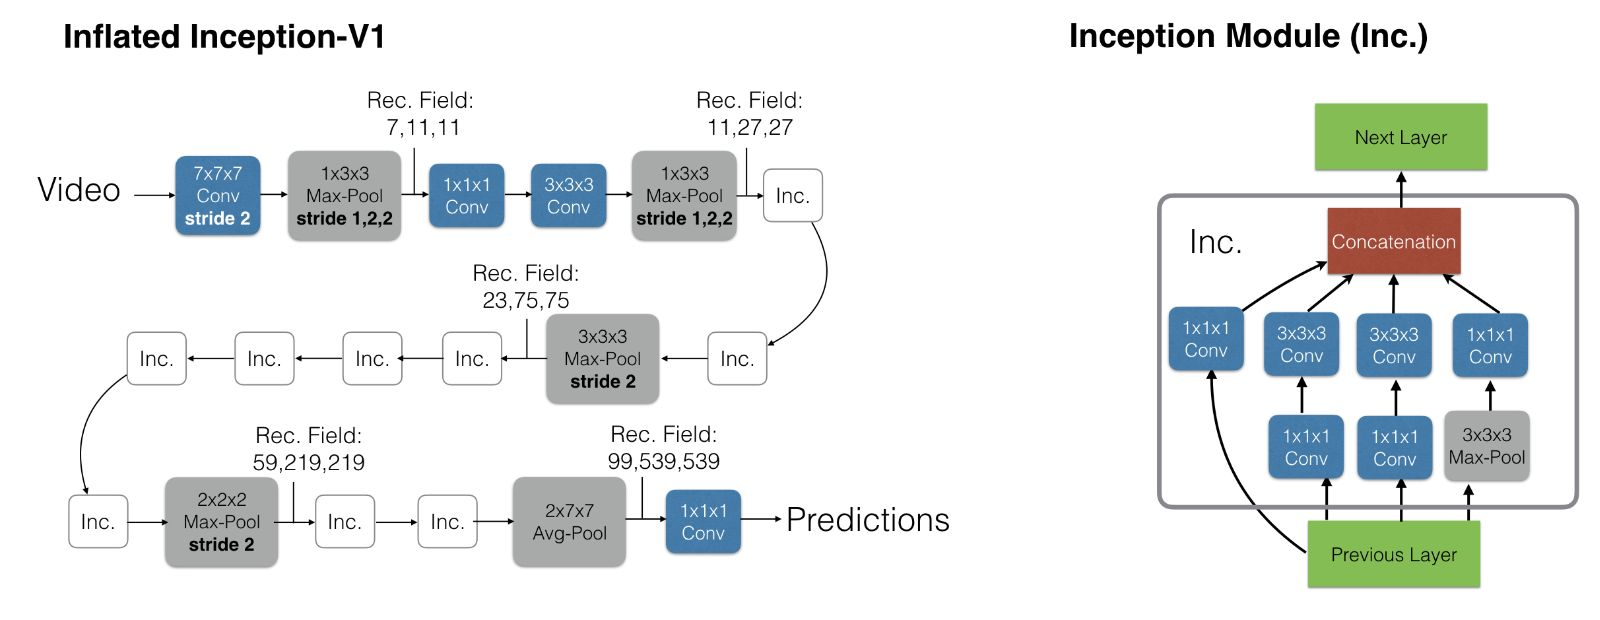
\includegraphics[width=12cm]{I3D}
	\centering
	\caption{The model architecture used in the I3D paper \cite{i3d}, where the Inflated Inception-V1 architecture (left) and it's detailed submodule (right) are shown.}
	\label{fig:I3D}
\end{figure}

%----------------------------------------------------------------------------------------
%	Modern
%----------------------------------------------------------------------------------------
\section{Model Evolution}

\begin{figure}[ht]
	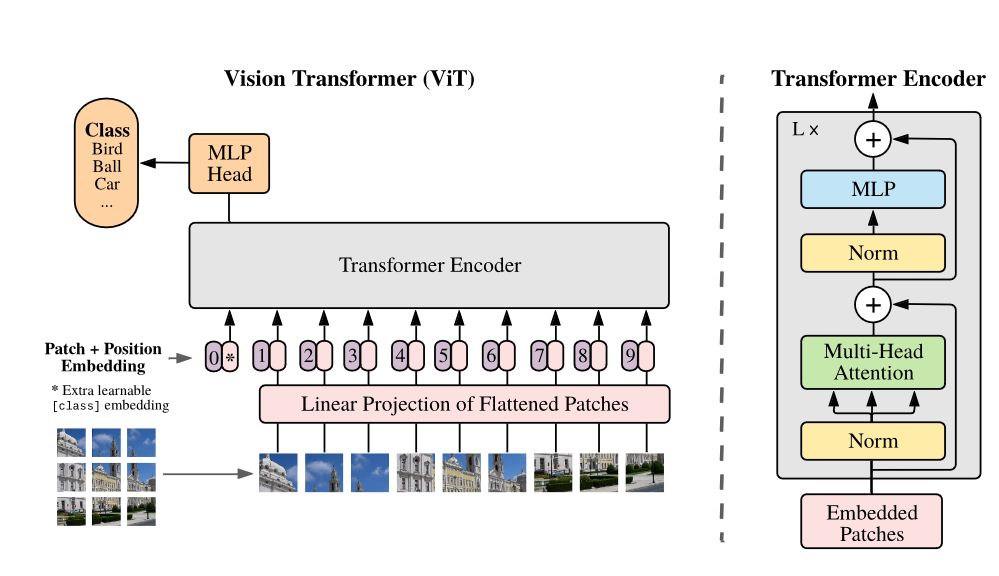
\includegraphics[width=10cm]{transformerActionRecognition}
	\centering
	\caption{The original transformer model proposed in \cite{transformer_og}, the image is split into fixed-size patches, linearly embed them, and add positional embeddings. It is then fed into a standard Transformer Encoder architecture.}
	\label{fig:transformerActionRecognition}
\end{figure}

\textbf{Transformers for Image Recognition at Scale} \cite{transformer_og}, extends beyond CNN's to explore transformer networks. While transformer networks are very easily applied to natural language processing tasks, it is not as easily applied to video and in particular action recognition. As depicted in figure \ref{fig:transformerActionRecognition}, the model utilizes a standard transformer architecture in order to learn features that are useful for action recognition. The goal of this being to leverage previously well studied NLP studies that indicate the attention features of transformers are useful for focusing on the relevant data. Figure \ref{fig:attentionExample} shows this effect, the goal of this being to mitigate the challenges of handling background data interference as previously described in section \ref{sec:challenges}. This logic is then further expanded upon in many future models to extend this functionality, such as \textbf{Multiview Transformers for Video Recognition} \cite{multiview_transformers} which explores using multiple separate encoders to explore multiple views.

\begin{figure}[ht]
	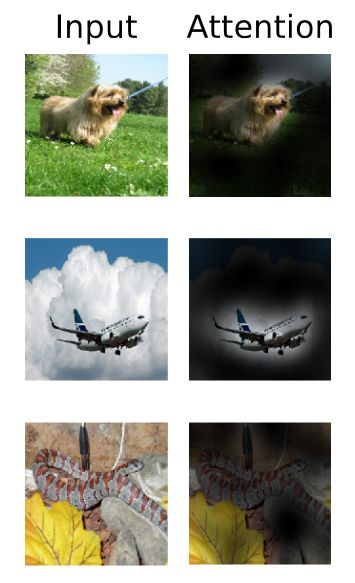
\includegraphics[width=5cm]{attentionExample}
	\centering
	\caption{Example feature outputs of how a transformer utilizes attention to focus on the main subject of a video in order to greater identify actions as shown in \cite{transformer_og}}
	\label{fig:attentionExample}
\end{figure}

%----------------------------------------------------------------------------------------
%	Datasets
%----------------------------------------------------------------------------------------
\section{Datasets}
\label{sec:datasets}

There are many action recognition datasets, some of which fit more specific use cases, and others which are more general and tailor to more in-the-wild data. For example the Charades dataset \cite{charades} focuses more on actions of people indoors and their interactions, whereas other datasets such as THUMOS \cite{THUMOS15} focus on many in-the-wild videos, where the location of the person can be different.

\textbf{The Kinetics Human Action Video Dataset} \cite{kinetics} is one of the primary in-the-wild action recognition datasets that are reported on by modern models. The primary advantage of this dataset over others that were published around the same time such as the UCF-101 dataset \cite{ucf101} is that as opposed to UCF's 101 classes and approximately 13,000 clips, the original kinetics dataset contained 400 classes and approximately 300,000 total clips which is magnitudes greater than other datasets of this type. This dataset has also been updated in 2020 to include 700 classes and over 600,000 clips. The extremely large amount of these clips, as well as containing all of; singular person actions (eg. headbanging, stretching), person-person actions (eg. handshake, tickling), and person-object actions (eg. riding a bike) among others creates a dataset that is difficult for a model to determine what action is being performed.

\begin{figure}[ht]
	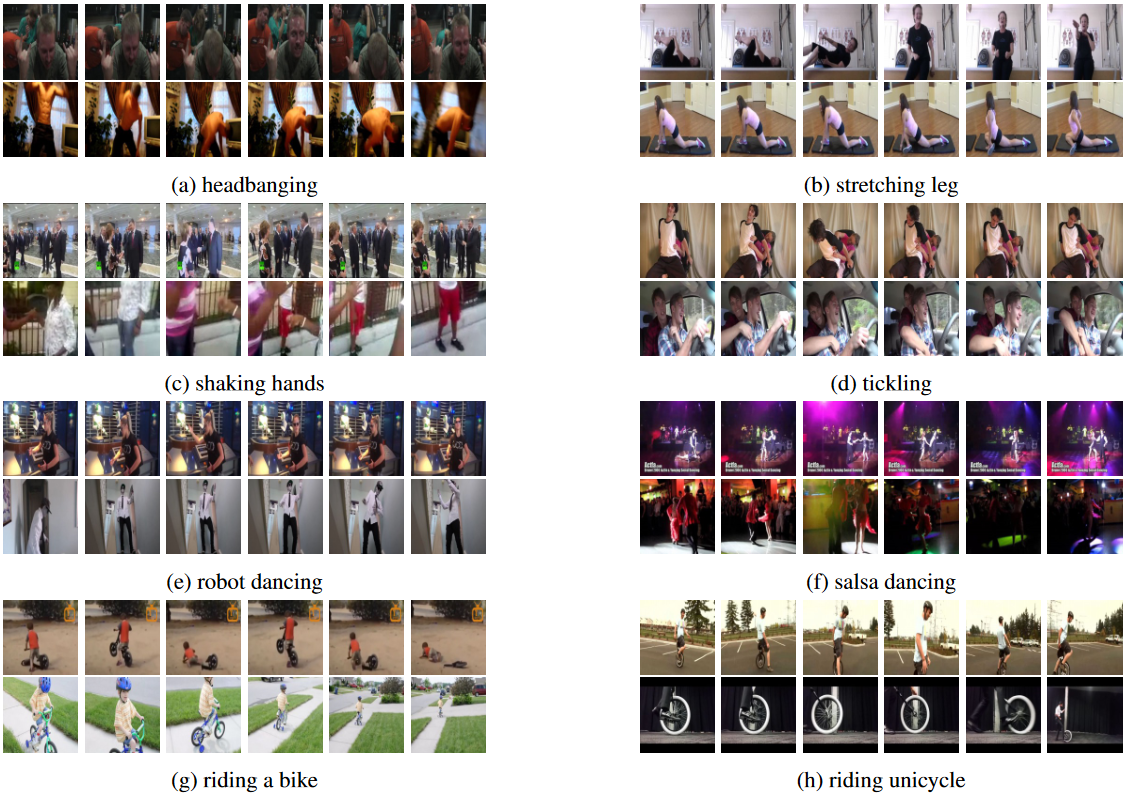
\includegraphics[width=13cm]{kinetics}
	\centering
	\caption{Example classes from the Kinetics dataset \cite{kinetics} which demonstrate the different singular person, person-person, and person-object interactions characterized in the dataset.}
	\label{fig:kinetics}
\end{figure}

\textbf{JHMDB} \cite{JHMDB} is the primary dataset that will be used in this paper. The JHMDB paper does not actually propose an entirely new dataset, rather it proposes a subset of the HMDB dataset \cite{hmdb}, with the addition of several features. While the dataset does offer more than only annotated poses, the main appeal of the dataset when considering the method used in this thesis is that they are fully annotated and adjusted poses to ensure that they are correct, meaning that the model can be independently be evaluated without having to consider the accuracy of the pose estimation model. Additionally, the dataset has been pruned such that the actions within the dataset only contain single person interactions, that lends itself very well to pose-based models, as generally only pose can be considered and the model can provide accurate results. Both of these features result in the dataset being highly popular with 2D-pose based models, and in particular models that create intermediate representations with these poses, as the data that is extracted from pose is both accurate and relevant to the action.

\begin{figure}[ht]
	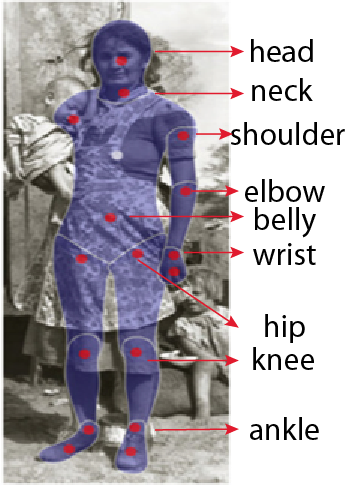
\includegraphics[width=5cm]{JHMDB}
	\includegraphics[width=6cm]{Pose JHMDB Indexes}
	\centering
	\caption{\textbf{Left:} JHMDB Annotated pose, each dot denoting a joint. \textbf{Right:} Simplified representation of this pose that will be used later in this thesis. Notably the foot joints are missing as they are not reliably labelled and are not used by the model. The indexes correspond to JHMDB joint indexes as if the subject were facing the camera.}
	\label{fig:JHMDB}
\end{figure}

%----------------------------------------------------------------------------------------
%	Pose Detection
%----------------------------------------------------------------------------------------
\section{Pose Detection}
\label{sec:pose-detection}

Throughout the majority of this thesis, and in some pose-based papers, the concept that there is some form of extracted pose from any given RGB frame is assumed to be accurate and complete. However, the extracting of these pose features, especially in the wild, is a difficult task in and of itself. This means that when considering pose-based models (as will be done further in section \ref{sec:pose-based}) that the accuracy of these techniques must be taken into account. Without an accurate pose model, it is impossible for these pose-based action recognition models to perform with any level of accuracy. Also worth noting is that some training data can have manually annotated pose data, an example being the previously discussed JHMDB dataset \cite{JHMDB}, which utilizes manually verified pose data. A very common model utilized by pose-based models is \textbf{OpenPose} \cite{openpose}, which as shown in figure \ref{fig:openpose}, is capable of detecting the poses of many people within the frame. In addition to what is shown in the figure, some models also utilize the joint heatmaps, which can also be easily generated by OpenPose. This is done through a modern technique using large CNN's and leveraging Part Affinity Fields, it is also allows for very fast real-time pose estimation.

\begin{figure}[ht]
	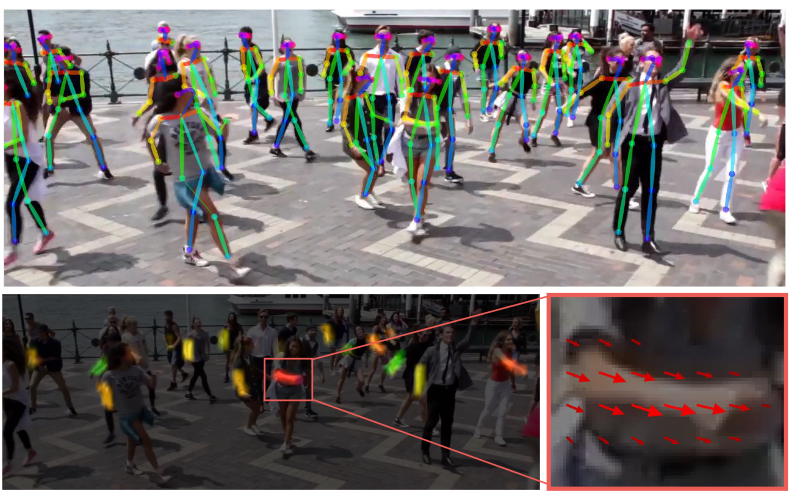
\includegraphics[width=12cm]{OpenPose}
	\centering
	\caption{Demonstrating the effectiveness of the OpenPose \cite{openpose} model. The \textbf{top} image showing that it is capable of distinguishing individual people, the \textbf{bottom left} showing the Part Affinity Fields corresponding to the limb connecting the right elbow and wrist. The \textbf{bottom right} shows a zoomed in view of these Part Affinity Fields.}
	\label{fig:openpose}
\end{figure}

There are many pose estimation models, as it is in itself a problem in the domain of computer vision that is constantly evolving. These can range from transformer based models such as ViTPose \cite{vitpose} designed to maximize dataset metrics, to the very lightweight models such as MoveNet developed by TensorFlow \cite{tensorflow2015-whitepaper}, developed for the purposes of real-time pose detection through mobile devices.

%----------------------------------------------------------------------------------------
%	Skeleton Based Models
%----------------------------------------------------------------------------------------
\section{Pose-Based Action Recognition}
\label{sec:pose-based}

Pose-based action recognition models have been well studied, and have been one of the popular forms of action recognition model as people typically determine actions by examining how a person is moving. This is because by focusing on the pose (sometimes referred to as the skeleton) of the person, you are able to effectively mitigate the background effects that were discussed in section \ref{sec:challenges}. This means that typically more lightweight models can be used as they are able to be pointed more towards the main subject rather than filter out background data. Of course this method also comes with challenges, notably that in testing in the wild, there must be effectively two models, one to extract the pose from the person(s) in the frame, and one to process this pose data and export an action. This can introduce another point of failure, but as discussed in section \ref{sec:pose-detection}, 2D pose detection has been consistently improving to the point that high quality pose data from fast models is the norm.

\begin{figure}[ht]
	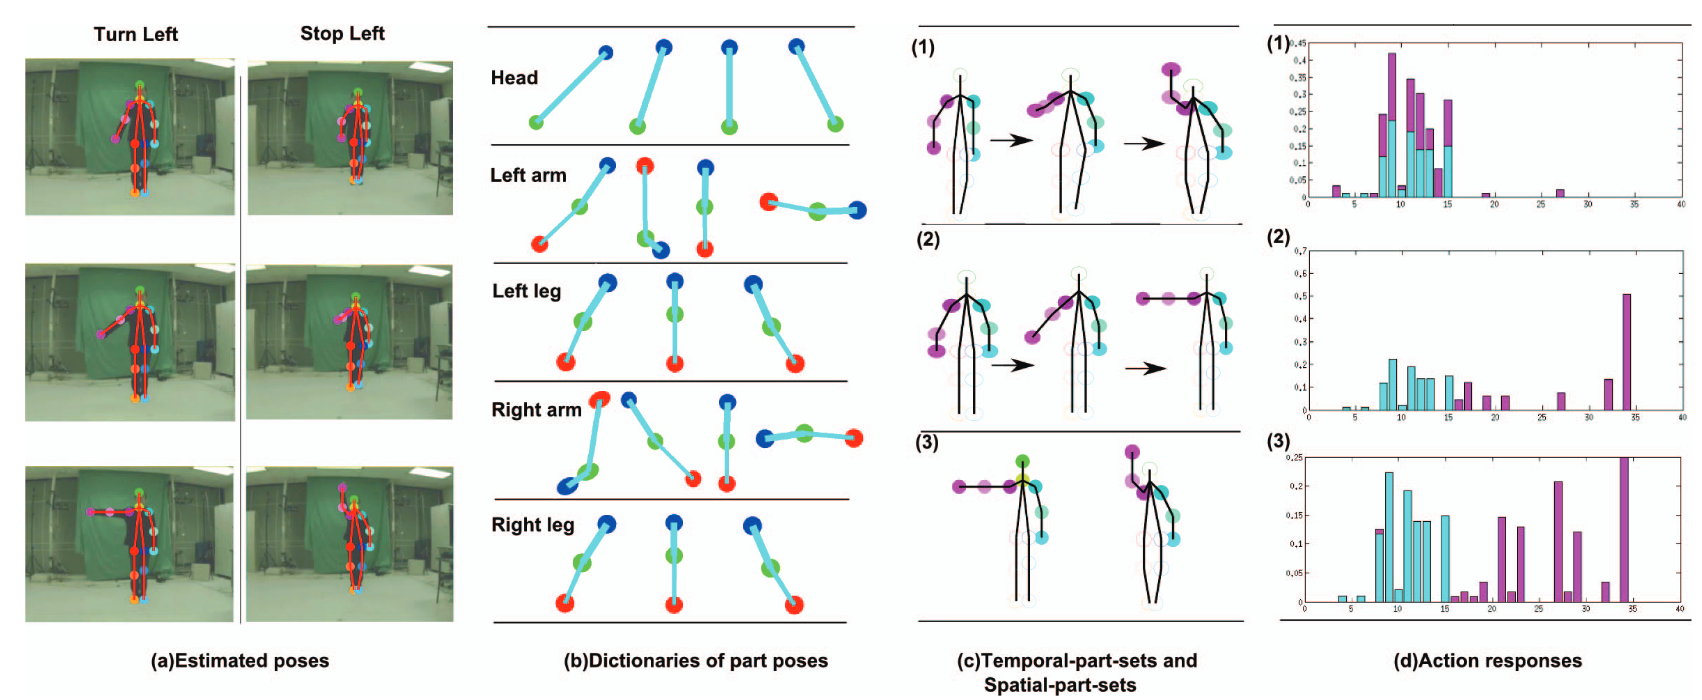
\includegraphics[width=12cm]{wangpose}
	\centering
	\caption{The overall framework of the action recognition model used by \textit{An approach to pose-based action recognition} \cite{WangPose}. \textbf{(a)} \& \textbf{(b)} show the esimated poses which are then used to create the dictionary of part poses. The temporal and spacial part sets in \textbf{(c)} are then represented in the histograms shown in \textbf{(d)}.}
	\label{fig:wangpose}
\end{figure}

\textbf{An approach to pose-based action recognition} \cite{WangPose} was a paper that proposed a technique to pose-based action recognition that did not utilize any of the typical popular CNN's that are used in modern models. Instead this model utilizes a dictionary of part poses that is then used by a bag-of-words model, a model typically geared towards the domain of NLP. This representation is shown in figure \ref{fig:wangpose}, and  while it performs well, it does suffer in that the bag-of-words models are not able to adapt to more sophisticated datasets.

\textbf{Pose-Based CNN Features for Action Recognition (P-CNN)} \cite{PCNN} is another model that utilizes the pose. Instead however, they use patches of the RGB frames centered on the various joints that have been detected, this is shown more in detail in figure \ref{fig:pcnn}. While this model does improve on typical models by using pose data, it does still struggle from the fact that it uses the raw RGB frame data, meaning that the model cannot be very small in order to handle this data.

\begin{figure}[ht]
	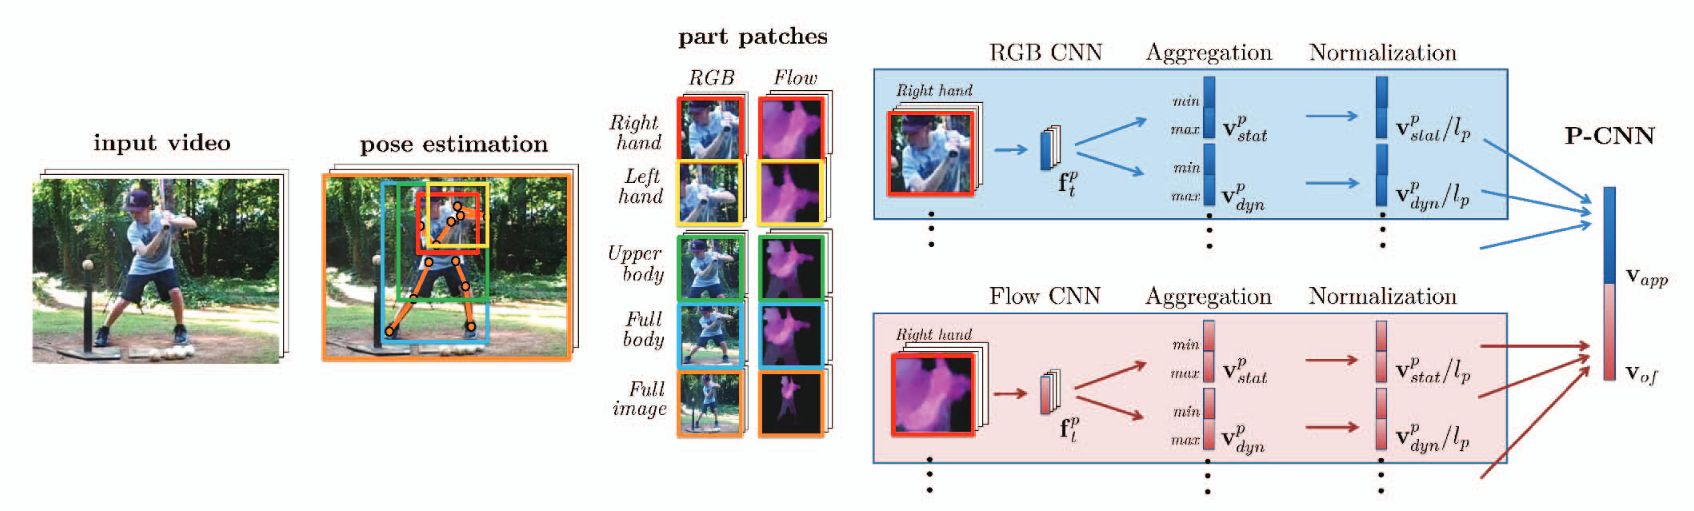
\includegraphics[width=12cm]{PCNN}
	\centering
	\caption{Illustration of P-CNN feature construction. RGB \& Optical Flow "Patches" are extracted around each joint, and sometimes containing multiple joints. These features are then passed through their respective CNN's, Aggregation, \& Normalization and then concatenated to form the final P-CNN feature.}
	\label{fig:pcnn}
\end{figure}

\begin{figure}[ht]
	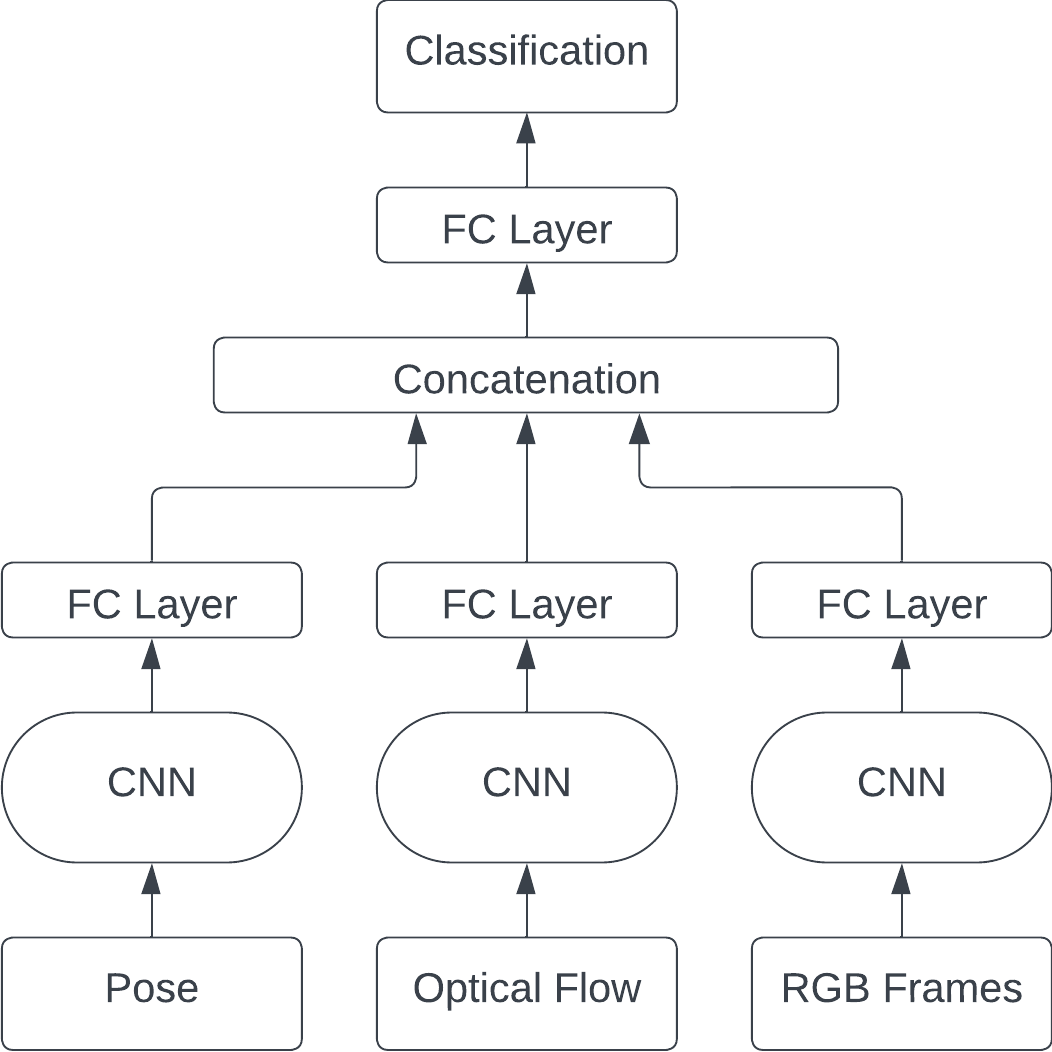
\includegraphics[width=6cm]{Fused}
	\centering
	\caption{A typical fused architecture. Each of the Pose, Optical Flow, and RGB Frames are passed through individual 3D-CNN's, the outputs are then concatenated to achieve a final output.}
	\label{fig:fused}
\end{figure}

Fusion-based architectures have had success in combining techniques used by basic 3D-CNN's, as seen in the I3D model \cite{i3d}, which as previously discussed in section \ref{sec:3dCNNModels} utilizes the RGB Frames \& Optical Flow in order to predict actions. Pose can be added to this architecture as shown in figure \ref{fig:fused}, where the pose data is added using some additional representation, the simple being the joint heatmaps exported from a previous model, and becoming more complex with intermediate representations that will be further discussed in section \ref{sec:intermediate}. \textbf{Chained Multi-stream Networks Exploiting Pose, Motion, and Appearance for Action Classification and Detection} \cite{Chained} is an addition to this type of model, where instead of the classic fused architecture, the model has individual loss functions added to each of the outputs, increasing performance while not adding very much additional complexity to the model.

\begin{figure}[ht]
	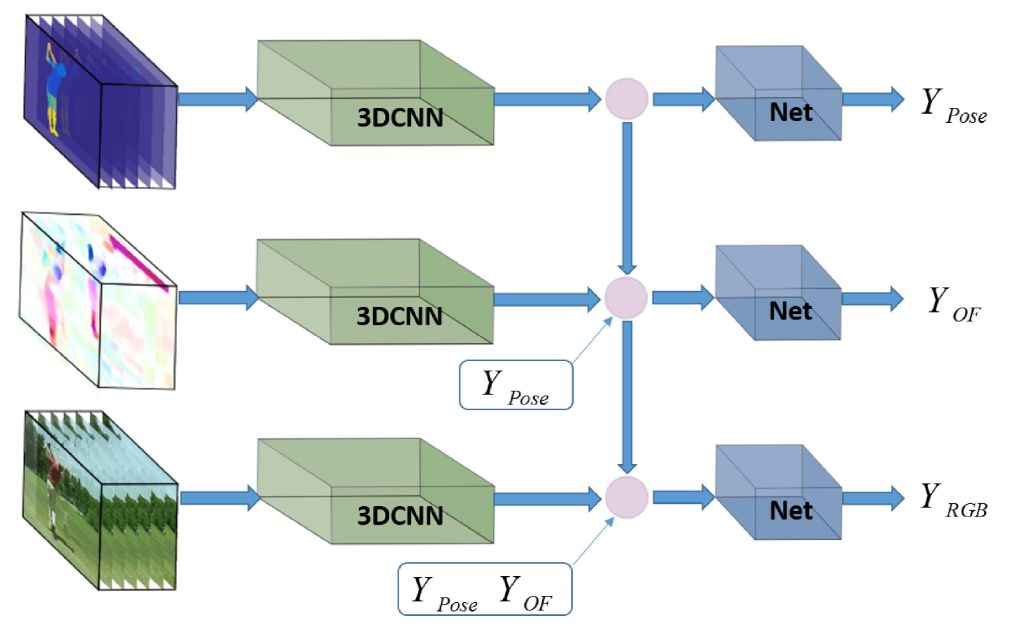
\includegraphics[width=5cm]{chained}
	\centering
	\caption{The chained architecture as shown in Chained Multi-stream Netowrks \cite{Chained}. The model differentiates in that it has separate loss functions for each of Pose, Optical Flow, and RGB, which are chained together in a way that they can be individually optimized.}
	\label{fig:chained}
\end{figure}

\subsection{Intermediate Representations}
\label{sec:intermediate}

Intermediate representations are the basis for what will be discussed in later sections of this thesis. Intermediate representations aim to reduce the pose data that has been extracted into simpler and more processable formats. This is generally done with the aim of using a much more lightweight model (sometimes 2D CNN rather than 3D) that requires significantly less computing power. Of course this kind of pre-processing comes with issues, notably that by converting the model into a format such as this, some data will inevitably be lost during the transition, so the problem definition shifts slightly to creating an intermediate representation that both allows for a lightweight model to be effectively trained on it and for the smallest amount of data to be lost in the transition.

\begin{figure}[ht]
	\includegraphics[width=12cm]{potionarchitecture}
	\centering
	\caption{The illustration of the PoTion representation \cite{potion}. The input joint heatmaps are colored based on their time in the frame, and the frames are then concatenated to form the final movement of the joint throughout the video.}
	\label{fig:potion-architecture}
\end{figure}

\textbf{Pose MoTion Representation for Action Recognition (PoTion)} \cite{potion} proposed one of these intermediate representations, however they did it in a way that was unique in that they only considered the joint positions rather than the skeletons themselves. Namely, the model utilizes the joint positions of a person throughout each frame of video to construct 2 dimensional images that reflect the movement of each of these joints. This is done by stacking each joint heatmap onto one image, and colorize them according to the point in time the frame is extracted. This colorization technique is shown in more detail in figure \ref{fig:potion-colourization}. The overall representation construction is shown in figure \ref{fig:potion-architecture}, and shows how after the colourization is performed, the heatmap images are then stacked together. These stacked images can then be passed into a simple 2D CNN, which can be quickly and efficiently trained and performs rather well. In the paper they also explore adding this implementation as another input to the I3D \cite{i3d} model in conjunction with the optical flow and rgb frames, which it showed to offer an increase in performance to the existing model. \textbf{Pose and Joint-Aware Action Recognition} \cite{poseandjointaware} is a slight improvement on this model structure, they utilize a similar colorization scheme. Instead of feeding all of the joints into the model, they developed a joint-motion re-weighting network (denoted in the paper as JMRN), which allowed for the model to easily find the dependencies between joints. This joint selection procedure allowed for the model to offer improved performance over the original PoTion model.

\begin{figure}[ht]
	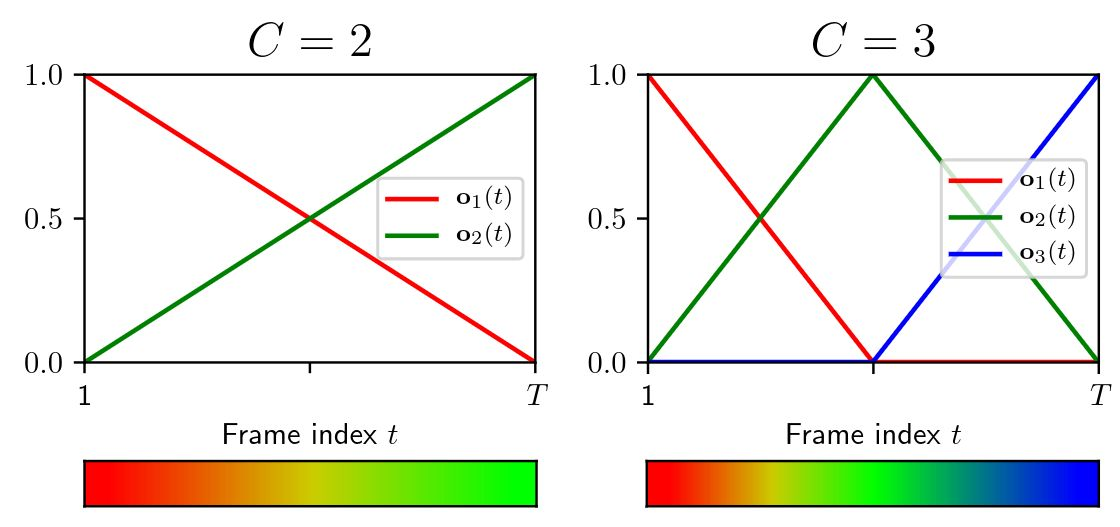
\includegraphics[width=10cm]{potionColorization}
	\centering
	\caption{The colourization method utilized by the PoTion model \cite{potion}. As the frame index moves throughout the video, the colour of the joint shifts from one to another. This can be done for any amount of colours, denoted by C, the figure shows examples for C=2 and C=3, but the same logic holds for more than 3.}
	\label{fig:potion-colourization}
\end{figure}

\textbf{Pose-Action 3D Machine for Video Recognition (PA3D)} \cite{PA3D} takes a similar approach to the PoTion model, but flavours it a bit differently. Similar to PoTion model, it leverages joint heatmaps similar to that exported from the OpenPose pose detection model, however it does not colorize the joints and aim to insert them into one image. A part of the model known as the \textit{Temporal Pose Convolution}, shown in figure \ref{fig:PA3D} is a core part of how the model functions. This is done through 1x1xN convolutions, which are run stacks of the joint heatmap images.

\begin{figure}[ht]
	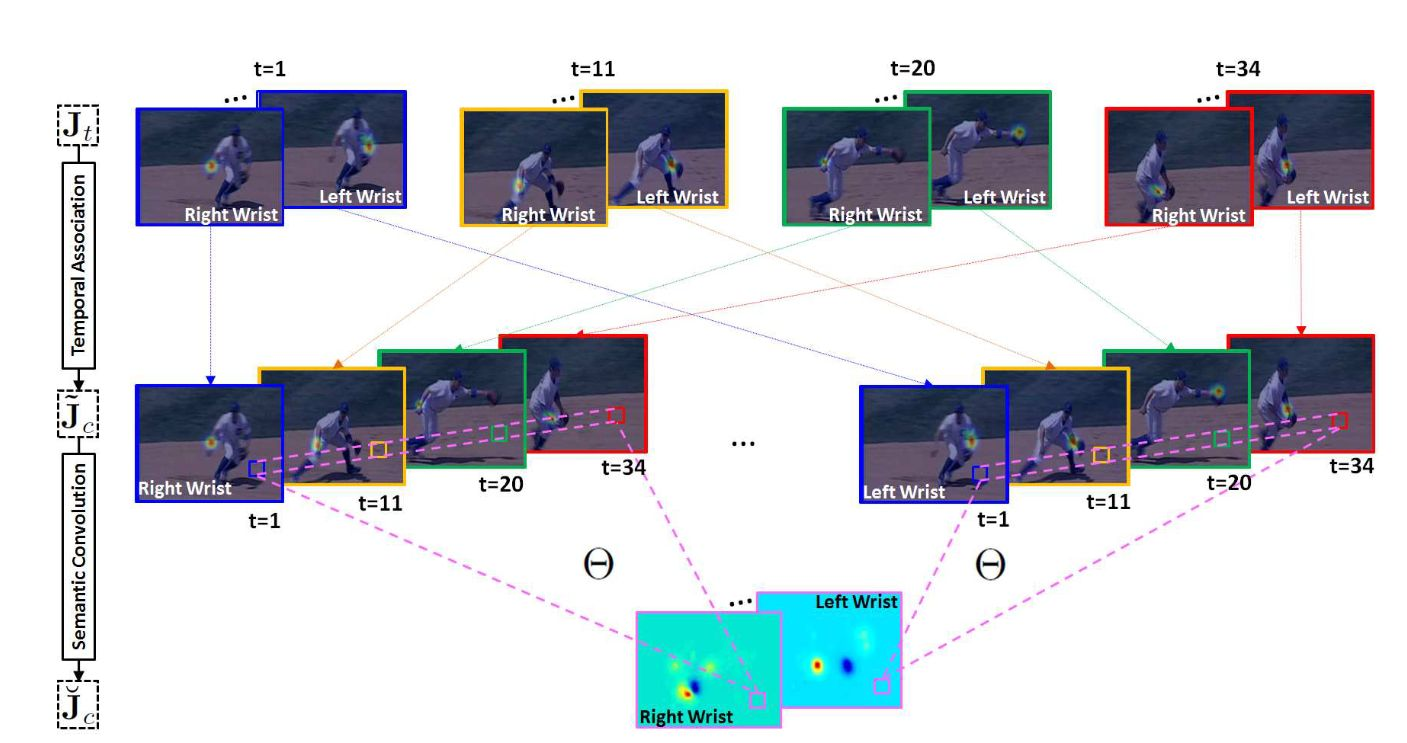
\includegraphics[width=12cm]{PA3D}
	\centering
	\caption{The main PA3D \cite{PA3D} model architecture, demonstrating the 1x1 convolutions used in order to construct the temporal cube.}
	\label{fig:PA3D}
\end{figure}

\textbf{Simple yet efficient real-time pose-based action recognition} \cite{simple_yet_efficient} was largely the inspiration for work done on this thesis. The goal of this paper was to provide a very lightweight and simple to understand intermediate representation that could be used by a very simple CNN to perform real-time action recognition. They do this by converting the skeletons into their unique \textit{Encoded Human Pose Image (EHPI)}, which is fundamentally just a 2d grid where the x-axis is frame index, and the y axis is the joint, this is shown in figure \ref{fig:EHPI}. This EHPI representation can then be used with a very simple CNN to provide very fast and good results in order to process actions in real time. There is one notable disadvantage in that it relies so heavily on the global positioning of the person in the frame. This means that the representation is very sensitive to things such as camera movement, where a slight movement results in the representation interpreting as the whole person sliding throughout the frame, however this could be mitigated via person detection to keep the person centered in the frame.

\begin{figure}[ht]
	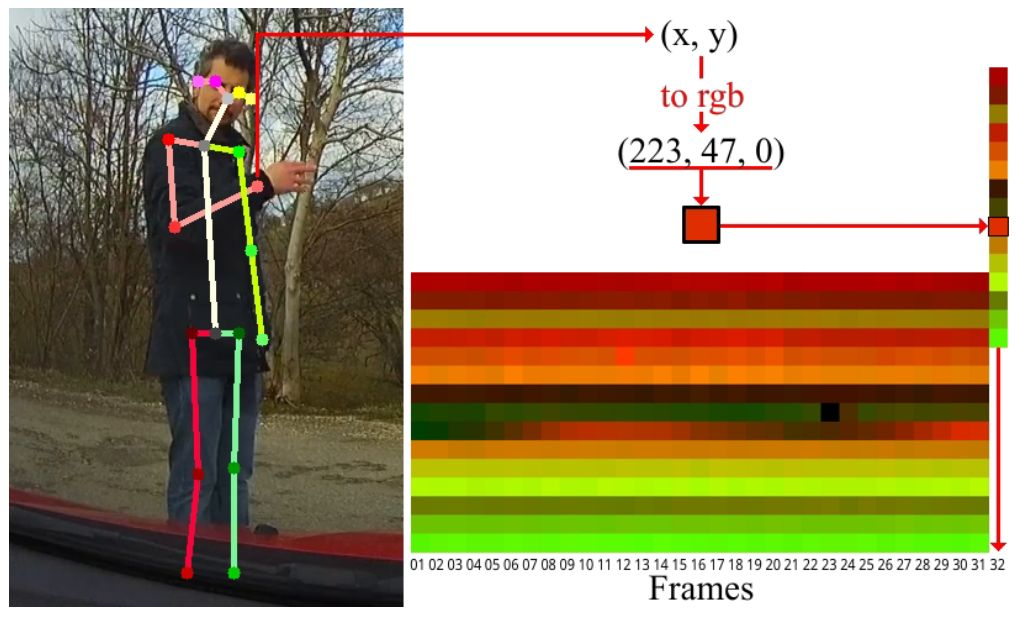
\includegraphics[width=12cm]{EHPI}
	\centering
	\caption{The EHPI representation used in the Simple yet efficient paper \cite{simple_yet_efficient}. The x, y coordinates of each joint are mapped to the red \& green values of a pixel, all joints are then stacked to form a column of joint positions in a frame. Each frame is then placed next to each other to form the 2D representation.}
	\label{fig:EHPI}
\end{figure}

\textbf{Make Skeleton-based Action Recognition Model Smaller, Faster and Better} \cite{smaller_faster_better} is yet another improvement on this intermediate representations, but with the particular focus on making the representations more resistant to both rotation \& shifting of a person throughout the frame.  As shown in figure \ref{fig:smallerfasterbetter}, this is done through two particular features, the cartesian coordinate feature which was used in previous models in a similar way \cite{simple_yet_efficient}, however it is done slightly differently through the JCD feature. The JCD feature is indifferent to rotations and shifting since all of the representation is aware of is the distance between any two given joints. This allows for easier generalization, however in the final model, both the cartesian coordinate and JCD features are used, as the authors determined that both were key in achieving high performance.

\begin{figure}[ht]
	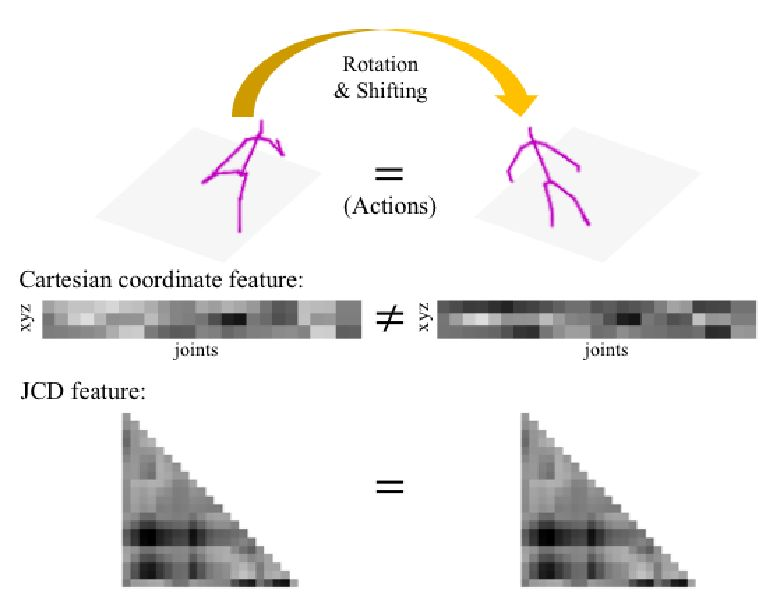
\includegraphics[width=8cm]{smallerfasterbetter}
	\centering
	\caption{The representation used by the Smaller, Faster, Better model \cite{smaller_faster_better}, this is split into two representations. The cartesian coordinates of each joint are encoded into a 2d representation, not dissimilar to previously discussed models \cite{simple_yet_efficient}. The JCD feature is a similar representation, but instead of x, y, and z coordinates, uses the distance between two joints.}
	\label{fig:smallerfasterbetter}
\end{figure}